% Created by tikzDevice version 0.8.1 on 2015-02-23 21:41:07
% !TEX encoding = UTF-8 Unicode
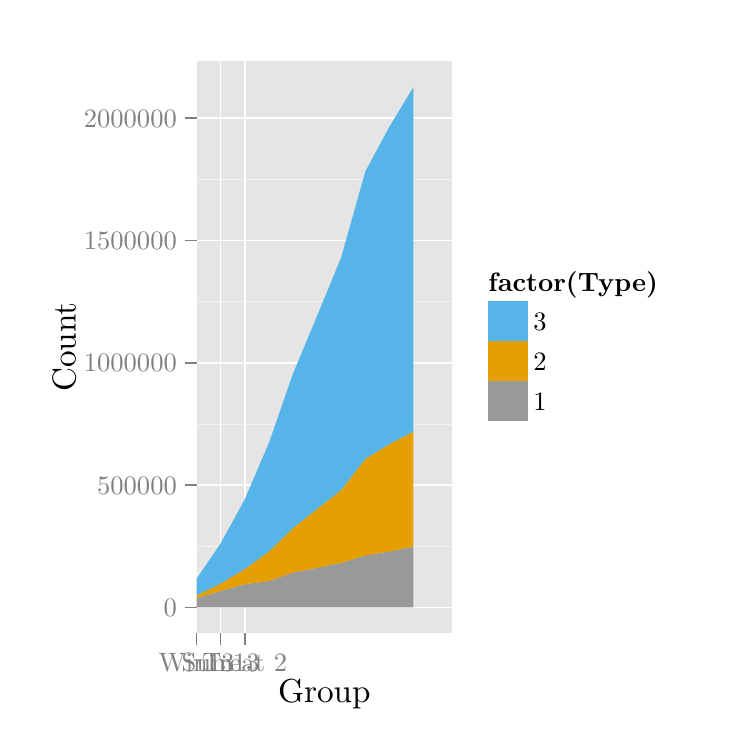
\begin{tikzpicture}[x=1pt,y=1pt]
\definecolor{fillColor}{RGB}{255,255,255}
\path[use as bounding box,fill=fillColor,fill opacity=0.00] (0,0) rectangle (252.94,252.94);
\begin{scope}
\path[clip] (  0.00,  0.00) rectangle (252.94,252.94);
\definecolor{drawColor}{RGB}{255,255,255}
\definecolor{fillColor}{RGB}{255,255,255}

\path[draw=drawColor,line width= 0.6pt,line join=round,line cap=round,fill=fillColor] (  0.00,  0.00) rectangle (252.94,252.95);
\end{scope}
\begin{scope}
\path[clip] ( 61.01, 34.03) rectangle (153.35,240.90);
\definecolor{fillColor}{gray}{0.90}

\path[fill=fillColor] ( 61.01, 34.03) rectangle (153.35,240.90);
\definecolor{drawColor}{gray}{0.95}

\path[draw=drawColor,line width= 0.3pt,line join=round] ( 61.01, 65.54) --
	(153.35, 65.54);

\path[draw=drawColor,line width= 0.3pt,line join=round] ( 61.01,109.74) --
	(153.35,109.74);

\path[draw=drawColor,line width= 0.3pt,line join=round] ( 61.01,153.94) --
	(153.35,153.94);

\path[draw=drawColor,line width= 0.3pt,line join=round] ( 61.01,198.14) --
	(153.35,198.14);
\definecolor{drawColor}{RGB}{255,255,255}

\path[draw=drawColor,line width= 0.6pt,line join=round] ( 61.01, 43.44) --
	(153.35, 43.44);

\path[draw=drawColor,line width= 0.6pt,line join=round] ( 61.01, 87.64) --
	(153.35, 87.64);

\path[draw=drawColor,line width= 0.6pt,line join=round] ( 61.01,131.84) --
	(153.35,131.84);

\path[draw=drawColor,line width= 0.6pt,line join=round] ( 61.01,176.04) --
	(153.35,176.04);

\path[draw=drawColor,line width= 0.6pt,line join=round] ( 61.01,220.25) --
	(153.35,220.25);

\path[draw=drawColor,line width= 0.6pt,line join=round] ( 61.01, 34.03) --
	( 61.01,240.90);

\path[draw=drawColor,line width= 0.6pt,line join=round] ( 69.73, 34.03) --
	( 69.73,240.90);

\path[draw=drawColor,line width= 0.6pt,line join=round] ( 78.44, 34.03) --
	( 78.44,240.90);
\definecolor{fillColor}{gray}{0.60}

\path[fill=fillColor] ( 61.01, 46.81) --
	( 69.73, 49.45) --
	( 78.44, 51.86) --
	( 87.15, 52.98) --
	( 95.86, 56.07) --
	(104.57, 57.80) --
	(113.28, 59.56) --
	(121.99, 62.25) --
	(130.70, 63.63) --
	(139.41, 65.48) --
	(139.41, 43.44) --
	(130.70, 43.44) --
	(121.99, 43.44) --
	(113.28, 43.44) --
	(104.57, 43.44) --
	( 95.86, 43.44) --
	( 87.15, 43.44) --
	( 78.44, 43.44) --
	( 69.73, 43.44) --
	( 61.01, 43.44) --
	cycle;
\definecolor{fillColor}{RGB}{230,159,0}

\path[fill=fillColor] ( 61.01, 47.78) --
	( 69.73, 52.08) --
	( 78.44, 57.34) --
	( 87.15, 63.63) --
	( 95.86, 72.15) --
	(104.57, 79.04) --
	(113.28, 85.87) --
	(121.99, 97.11) --
	(130.70,102.47) --
	(139.41,107.02) --
	(139.41, 65.48) --
	(130.70, 63.63) --
	(121.99, 62.25) --
	(113.28, 59.56) --
	(104.57, 57.80) --
	( 95.86, 56.07) --
	( 87.15, 52.98) --
	( 78.44, 51.86) --
	( 69.73, 49.45) --
	( 61.01, 46.81) --
	cycle;
\definecolor{fillColor}{RGB}{86,180,233}

\path[fill=fillColor] ( 61.01, 53.75) --
	( 69.73, 66.58) --
	( 78.44, 82.49) --
	( 87.15,102.81) --
	( 95.86,127.91) --
	(104.57,148.78) --
	(113.28,169.89) --
	(121.99,200.95) --
	(130.70,217.13) --
	(139.41,231.50) --
	(139.41,107.02) --
	(130.70,102.47) --
	(121.99, 97.11) --
	(113.28, 85.87) --
	(104.57, 79.04) --
	( 95.86, 72.15) --
	( 87.15, 63.63) --
	( 78.44, 57.34) --
	( 69.73, 52.08) --
	( 61.01, 47.78) --
	cycle;
\end{scope}
\begin{scope}
\path[clip] (  0.00,  0.00) rectangle (252.94,252.94);
\definecolor{drawColor}{gray}{0.50}

\node[text=drawColor,anchor=base east,inner sep=0pt, outer sep=0pt, scale=  0.96] at ( 53.90, 40.13) {0};

\node[text=drawColor,anchor=base east,inner sep=0pt, outer sep=0pt, scale=  0.96] at ( 53.90, 84.33) {500000};

\node[text=drawColor,anchor=base east,inner sep=0pt, outer sep=0pt, scale=  0.96] at ( 53.90,128.54) {1000000};

\node[text=drawColor,anchor=base east,inner sep=0pt, outer sep=0pt, scale=  0.96] at ( 53.90,172.74) {1500000};

\node[text=drawColor,anchor=base east,inner sep=0pt, outer sep=0pt, scale=  0.96] at ( 53.90,216.94) {2000000};
\end{scope}
\begin{scope}
\path[clip] (  0.00,  0.00) rectangle (252.94,252.94);
\definecolor{drawColor}{gray}{0.50}

\path[draw=drawColor,line width= 0.6pt,line join=round] ( 56.75, 43.44) --
	( 61.01, 43.44);

\path[draw=drawColor,line width= 0.6pt,line join=round] ( 56.75, 87.64) --
	( 61.01, 87.64);

\path[draw=drawColor,line width= 0.6pt,line join=round] ( 56.75,131.84) --
	( 61.01,131.84);

\path[draw=drawColor,line width= 0.6pt,line join=round] ( 56.75,176.04) --
	( 61.01,176.04);

\path[draw=drawColor,line width= 0.6pt,line join=round] ( 56.75,220.25) --
	( 61.01,220.25);
\end{scope}
\begin{scope}
\path[clip] (  0.00,  0.00) rectangle (252.94,252.94);
\definecolor{drawColor}{gray}{0.50}

\path[draw=drawColor,line width= 0.6pt,line join=round] ( 61.01, 29.77) --
	( 61.01, 34.03);

\path[draw=drawColor,line width= 0.6pt,line join=round] ( 69.73, 29.77) --
	( 69.73, 34.03);

\path[draw=drawColor,line width= 0.6pt,line join=round] ( 78.44, 29.77) --
	( 78.44, 34.03);
\end{scope}
\begin{scope}
\path[clip] (  0.00,  0.00) rectangle (252.94,252.94);
\definecolor{drawColor}{gray}{0.50}

\node[text=drawColor,anchor=base,inner sep=0pt, outer sep=0pt, scale=  0.96] at ( 61.01, 20.31) {Win13};

\node[text=drawColor,anchor=base,inner sep=0pt, outer sep=0pt, scale=  0.96] at ( 69.73, 20.31) {Sum13};

\node[text=drawColor,anchor=base,inner sep=0pt, outer sep=0pt, scale=  0.96] at ( 78.44, 20.31) {Treat 2};
\end{scope}
\begin{scope}
\path[clip] (  0.00,  0.00) rectangle (252.94,252.94);
\definecolor{drawColor}{RGB}{0,0,0}

\node[text=drawColor,anchor=base,inner sep=0pt, outer sep=0pt, scale=  1.20] at (107.18,  9.03) {Group};
\end{scope}
\begin{scope}
\path[clip] (  0.00,  0.00) rectangle (252.94,252.94);
\definecolor{drawColor}{RGB}{0,0,0}

\node[text=drawColor,rotate= 90.00,anchor=base,inner sep=0pt, outer sep=0pt, scale=  1.20] at ( 17.30,137.47) {Count};
\end{scope}
\begin{scope}
\path[clip] (  0.00,  0.00) rectangle (252.94,252.94);
\definecolor{fillColor}{RGB}{255,255,255}

\path[fill=fillColor] (162.22,106.40) rectangle (232.03,168.54);
\end{scope}
\begin{scope}
\path[clip] (  0.00,  0.00) rectangle (252.94,252.94);
\definecolor{drawColor}{RGB}{0,0,0}

\node[text=drawColor,anchor=base west,inner sep=0pt, outer sep=0pt, scale=  0.96] at (166.49,157.64) {\bfseries factor(Type)};
\end{scope}
\begin{scope}
\path[clip] (  0.00,  0.00) rectangle (252.94,252.94);
\definecolor{drawColor}{RGB}{255,255,255}
\definecolor{fillColor}{gray}{0.95}

\path[draw=drawColor,line width= 0.6pt,line join=round,line cap=round,fill=fillColor] (166.49,139.57) rectangle (180.94,154.03);
\end{scope}
\begin{scope}
\path[clip] (  0.00,  0.00) rectangle (252.94,252.94);
\definecolor{fillColor}{RGB}{86,180,233}

\path[fill=fillColor] (166.49,139.57) rectangle (180.94,154.03);

\path[] (166.49,139.57) --
	(180.94,154.03);
\end{scope}
\begin{scope}
\path[clip] (  0.00,  0.00) rectangle (252.94,252.94);
\definecolor{drawColor}{RGB}{255,255,255}
\definecolor{fillColor}{gray}{0.95}

\path[draw=drawColor,line width= 0.6pt,line join=round,line cap=round,fill=fillColor] (166.49,125.12) rectangle (180.94,139.57);
\end{scope}
\begin{scope}
\path[clip] (  0.00,  0.00) rectangle (252.94,252.94);
\definecolor{fillColor}{RGB}{230,159,0}

\path[fill=fillColor] (166.49,125.12) rectangle (180.94,139.57);

\path[] (166.49,125.12) --
	(180.94,139.57);
\end{scope}
\begin{scope}
\path[clip] (  0.00,  0.00) rectangle (252.94,252.94);
\definecolor{drawColor}{RGB}{255,255,255}
\definecolor{fillColor}{gray}{0.95}

\path[draw=drawColor,line width= 0.6pt,line join=round,line cap=round,fill=fillColor] (166.49,110.67) rectangle (180.94,125.12);
\end{scope}
\begin{scope}
\path[clip] (  0.00,  0.00) rectangle (252.94,252.94);
\definecolor{fillColor}{gray}{0.60}

\path[fill=fillColor] (166.49,110.67) rectangle (180.94,125.12);

\path[] (166.49,110.67) --
	(180.94,125.12);
\end{scope}
\begin{scope}
\path[clip] (  0.00,  0.00) rectangle (252.94,252.94);
\definecolor{drawColor}{RGB}{0,0,0}

\node[text=drawColor,anchor=base west,inner sep=0pt, outer sep=0pt, scale=  0.96] at (182.75,143.50) {3};
\end{scope}
\begin{scope}
\path[clip] (  0.00,  0.00) rectangle (252.94,252.94);
\definecolor{drawColor}{RGB}{0,0,0}

\node[text=drawColor,anchor=base west,inner sep=0pt, outer sep=0pt, scale=  0.96] at (182.75,129.04) {2};
\end{scope}
\begin{scope}
\path[clip] (  0.00,  0.00) rectangle (252.94,252.94);
\definecolor{drawColor}{RGB}{0,0,0}

\node[text=drawColor,anchor=base west,inner sep=0pt, outer sep=0pt, scale=  0.96] at (182.75,114.59) {1};
\end{scope}
\end{tikzpicture}
